\chapter{Backround}\label{ch:background}

In this chapter, we introduce the theoretical
background for our implementation, especially regarding the Secure Shared Folder 
(SSF) scheme. We introduce some notation (\cref{sc:notation}) and
describe existing cryptographic primitives (\cref{sc:DKR}, \cref{sc:SSKG}, \cref{sc:CGKA})
that are used in the scheme.
We also give an informal description of the novel primitives 
underlying the SSF scheme and their operations (\cref{sc:SSF}).
An informal description of the scheme closes the section (\cref{sc:SSF-scheme}).

A section on related work is also included (\cref{sc:related-work}),
to discuss further research related to this thesis but not specifically 
part of the theoretical background needed to understand the SSF construction.

\section{Notation}\label{sc:notation}

We assume the following conventions:
\begin{itemize}
    \item Intervals are inclusive, i.e., $[a, b] = \{x \in \mathbb{N} \mid a \leq x \leq b\}$.
    \item A sequence of elements of length $n$ starts at index $0$ and ends at index $n-1$, as in common practice in programming languages.
    \item \texttt{Monospace font} is used for references to pseudocode and code references in running text.
\end{itemize}

\section{Double-PRF}\label{sc:DPRF}

A pseudorandom function family (PRF) $F$ is a collection of functions
with two arguments $x$ and $y$, respectively a key and a message
represented as bit strings, which returns bit string $z$ as output.
Informally we think of a PRF as being \textit{secure} if, for any given $x$
uniformly sampled from the key space, the function of one argument
$F_x(y) = F(x, y)$ is indistinguishable from a random function, i.e.
an efficient adversary cannot distinguish with significant advantage
between a function chosen at random from the PRF family and a random oracle.
A \textit{swap-PRF} is a PRF where swapping the keys for the messages
still result in indistinguishability from random~\cite{EPRINT:BelLys15}.
When $F$ is both a PRF and a swap-PRF, it is called a \textit{dual-PRF}.
As analysed and proved by Backendal et al.~\cite{C:BBGS23} HMAC is not always a
dual-PRF. However, if fixed-length keys are used, no matter the length,
then it is provably a dual-PRF.

The \textit{double-PRF} security notion by Backendal et al.
is slightly stronger than dual-PRF security.
It requires the function family to be indistinguishable from a random 
function not only when keyed either by the first input or the second input
but as well as when keyed through both inputs at the same time.
This means that an adversary simultaneously have access to both 
oracles for the PRF and its swap-PRF.
They also show that double-PRF security is implied by dual-PRF security,
thus HMAC is a double-PRF in case of fixed-length keys.
See \cref{sc:ssf-double-prf} for details on the implementation of double-PRF in SSF.

\section{Dual-Key Regression}\label{sc:DKR}

\begin{figure}
    \centering
    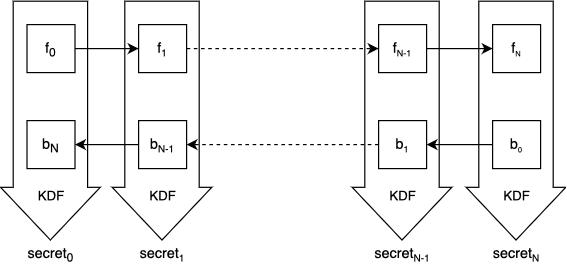
\includegraphics[width=0.8\textwidth]{figures/dkr.drawio.png}
    \caption{Dual-Key Regression (DKR), displaying the forward and backward chains and corresponding sequence of secrets derived through the application of the KDF. }
    \label{fig:dkr}
\end{figure}

A hash chain is a sequence of values
$h_{0}, ..., h_{n}$ which starting from an initial
element $h_0$ progresses by iteratively calculating
a given hash function $H$ on the predecessor,
i.e., given $h_i$, the next element $h_{i+1}$ is computed as $h_{i+1} = H(h_i)$.
Due to the pre-image resistance of the hash function $H$, 
it is computationally hard to find $h_i$ given $h_{i+1}$.
We call an ``interval'' $[a, b]$ a subsequence of elements
of a hash chain starting from index $a$ and ending
on index $b$ inclusive of the chain.
Dual-key regression (DKR) introduced by Shafagh et al.~\cite{USENIX:SBRH20} is a
cryptographic primitive based on hash chains, that
allows sharing a potentially very large interval 
of secrets by only sharing a small state.
Dual-key regression (\cref{fig:dkr}) uses a pair of hash chains,
a ``forward'' and ``backward'' chain, with an additional
parameter $N$ denoting the
upper bound on the maximum length of each chain.
A forward chain is just a hash chain as defined
above, $f_{0}, ..., f_{N}$.
A backward chain instead is a hash chain, of which the
elements are released in reverse order of computation
$b_{N}, ..., b_{0}$, meaning that the element of the chain 
at index $i$ will be the element calculated by $N - i$
iterations of the hash function on the initial $b_{0}$
element. We notice that the DKR upper bound parameter
$N$ is imposed by the
fact that elements of the backward chains are taken in
reverse order and the hash function cannot be inverted.
Finally, a DKR secret is calculated by applying
a key derivation function (KDF) that takes
as input elements from both chains at the same
time corresponding to the same index, i.e.\!
elements $f_{i}$ and $b_{(N - i)}$.
The KDF we will use will be a double-PRF (\cref{sc:DPRF}, \cref{sc:ssf-double-prf}).


\section{Seekable Sequential Key Generators}\label{sc:SSKG}

Seekable Sequential Key Generators (SSKG) are cryptographic objects introduced by Marson et al.~\cite{ESORICS:MarPoe13}.
They are sequential pseudo random generators (SRG) with additional properties.
A sequential random generator is a stateful pseudo random generator (PRG)~\cite{cryptoeprint:2017/208}, 
which outputs a fixed-length string for each invocation, 
thus producing a sequence of pseudo random strings through multiple invocations.
A SRG is said to be secure if its output is indistinguishable from a uniformly random sampled string.
SSKG are SRG with the additional property of being seekable,
meaning that they offer a convenient operation to compute the
element at a certain offset in the sequence from the initial one.
This operation is called \texttt{Seek} and runs in sublinear time.

SSKG are widely used in practice:
the logging service of the \texttt{systemd} system manager,
which is a core component in many Linux-based operating systems,
is using them to power fast verification of arbitrary log entries against tampering.
SSKG are provably (forward-)secure in the standard model, i.e.,
an adversary gets no advantage from learning current output of the SSKG
while trying to compute the past outputs.
SSKG can be seen as time-efficient alternatives to hash chains (\cref{sc:DKR}),
when the \texttt{Seek} operation is required.
Marson et al.\ propose two constructions: one is based on number theory~\cite{ESORICS:MarPoe13}
and the other one uses a tree-based construction~\cite{ESORICS:MarPoe14}.
The latter suffers a logarithmic space overhead 
compared to the constant space required to store 
only the starting element of a hash chain.
However, in our implementation we will be using the later tree-based version of SSKG~\cite{ESORICS:MarPoe14}
because it allows seeking also starting from any point in the sequence
instead of just from the initial element.
We discuss the practical details more in-depth in \cref{sc:ssf-sskg}.

\section{Continuous Group Key Agreement}\label{sc:CGKA}

A continuous group key agreement (CGKA) scheme~\cite{C:ACDT20}
allows a long-lived, dynamic, asynchronous group of users to agree 
continuously on shared symmetric secrets.
The shared group secret is recomputed both as users add (remove)
other members to (resp.\ from) the group, and when users periodically
refresh their private secret state. These operations can happen
asynchronously, allowing group members to refresh their 
state without requiring all other members to be online 
simultaneously.
CKGA allows a group of $n$ users to perform the above critical 
operations in $\log(n)$ time,
thus it can be used in practice with a large number of members.
The primitive guarantees post-compromise security (PCS) and forward secrecy (FS):
in case of a compromise in which a user's secret is leaked
to an adversary the group keys should shortly become private
again through the ordinary protocol state refreshes; the past
group keys remain secure as well.

A first ends-to-ends\footnote{While in communication protocols between two entities (where an entity is commonly referred to as endpoint) we normally speak about end-to-end encryption, in case of a group setting we use the plural form for the term.}
encrypted (E2EE) primitive for an asynchronous group key exchange 
has been introduced by Cohn-Gordon et al.~\cite{CCS:CCGMM18}.The research was conducted to address the scenario of secure group messaging.
In such a case multiple users want to exchange messages, asynchronously
between them securely, which can be reduced to the problem
of asynchronously agreeing on a shared symmetric key.
The authors presented a way to achieve PCS in such cases.
To this end they designed the Asynchronous Ratcheting Trees (ART),
which is internally using a Diffie-Hellman tree~\cite{10.1145/1368310.1368347} 
to represent the public and private secrets for each user
and derive a shared secret from them. In Diffie-Hellman
trees, the user keypair is stored in the leaves.
This primitive offers the operations to add and remove members
as well as refreshing a user's own secret efficiently in $\log(n)$ time.
It has been of significant interest in the industry and
got a dedicated working groups by the IETF.
The ART construction has been replaced by the TreeKEM
construction proposed by Bhargavan et al.~\cite{TreeKEM}.
In TreeKEM, members are organised in a tree-shaped structure
as in ART, however the keys stored in the tree for each group
can be any keypair supporting key encapsulation (KEM).
The key advantage of TreeKEM over ART is that
most operations are ``mergeable'':
any device receiving two
concurrent operations will be able to process and execute both of them,
instead of executing one and refuses the other.
Alwen et al.~\cite{C:ACDT20} slightly modified the TreeKEM construction
to achieve \textit{optimal} security in the context of
secure group messaging.
Further refinements for efficiency and security have 
been studied in recent years under different assumptions and threat models~\cite{TCC:ACJM20, SP:KPWKCCMYAP21, CCS:ACDT21, CCS:AHKM22, EC:AANKPPW22, C:AlwJosMul22, C:AlwMulTse23, IWSPA:KEONO23}.

Of particular interest is the family of CGKA protocols called admin-CGKA (A-CGKA).
In this declination of CGKA, a subgroup of the users are admins. 
Admins can perform additional operations that are otherwise disallowed, such as removing other members of the group.

As we will see in \cref{sc:SSF-scheme}, our secure shared folder (SSF) scheme uses A-CGKA as a building block
inside the GKP scheme (\cref{sc:gkp-scheme}).
The specific version of A-CGKA we use, called dual-CGKA, is composed of a CGKA within CGKA to manage the admin state, as proposed by
B{\'a}lbas et al.\!~\cite{USENIX:BalColVau23}.

\section{Messaging Layer Security}\label{sc:MLS}

As already discussed in \cref{sc:CGKA}, a major application of CGKA is in the field of group messaging.
The messaging layer security (MLS) protocol from IETF~\cite{rfc9420},
a standardised protocol for secure group messaging, is indeed 
built on top of CGKA. CGKA is used to agree on a shared symmetric key
to later derive message encryption keys.

CGKA instantiations rely on message exchange
between the members of the group to actually perform the protocol operations.
Therefore, it is not surprising that most of the implementations
of CGKA come from libraries that also implement the MLS protocol (\cref{sc:CGKA-implementations}).
The messages needed for the CGKA operations are referred to ``control'' messages in the context of MLS.
CGKA operations are based on a proposal and commit mechanism,
where (multiple) users can propose (multiple) group state updates
through proposal messages and then commit to them through a commit message
sent by one member, referring to a list of previously shared proposals. 
The proposals are of different types and model the operation of adding or removing 
members as well as refreshing a user's secret state, as seen above (\cref{sc:CGKA}).
The commit messages are used to agree and finalise the state updates,
thus helping to synchronize the group state among the members.

The MLS protocol specification also offers an abstract overview of
the component and architecture of a system using it, 
where the concept of a ``delivery service''
(DS) is introduced. The DS is a facilitator component that is used to 
deliver the messages between the members of the group and helps in
synchronising the group state. The DS is assumed to reliably
send the messages to the group members in order, so that the
group is able to advance the CGKA cryptographic state reliably.
However, the DS is not part of CGKA itself,
but it is a necessary component to implement the scheme in practice.
Further, the MLS protocol offers a way to securely exchange ``application messages''
on top of CGKA. The application messages are just opaque messages
without any predefined structure or semantic, in contrast to the
CGKA control messages.
Application messages are encrypted with a key derived from the shared group secret.

As we will see in \cref{ch:setup}, we use a library implementing MLS and not just CGKA in our implementation of SSF.
We will make use of some additional features from MLS that are not part of CGKA, such as the
aforementioned encrypted application messages,
and take inspiration from the system architecture of MLS for our own architecture design.
We discuss the architecture in further details in \cref{ch:setup}.

\section{Secure Shared Folder Building Blocks}\label{sc:SSF}

In this section we describe the
contributions from~\cite{GKP}
which are going to be used
in the SSF scheme.
We start by recalling the novel security notion for persistent
data called interval access security (IAC) (\cref{sc:iac}).
Then we describe the generalised dual-key regression and group key progression primitives
(\cref{sc:background-generalised-DKR,sc:gkp-scheme}).

\subsection{Novel Security Notion for Persistent Data: Interval Access Security}\label{sc:iac}

The SSF (\cref{sc:mental-model}) is a new primitive that targets a novel security 
notion for persistent data shared among a dynamic 
group of users: interval access control (IAC).
The new security notion aims to better and more naturally
capture the minimal security for shared persistent data.

In short, IAC requires that a user can only decrypt data that
is shared in the time frame in which the user is a member
of the group. For data in transit, the data is regarded as
ephemeral and therefore the creation and sharing of the data
itself is naturally bound to the point in time of the exchange,
and to its deletion. Persistent data on the other hand, naturally
outlive the moment in time in which it is shared.
Therefore, the lifetime of data at rest is decoupled from the
lifetime of the user access to the group exchanging the data.
Thus, a user that receives access to some data while being the
member of a group, will be able to still decrypt the data
after he looses membership, unless the data is re-encrypted
and the old ciphertext is securely deleted, because data
persistence prevents automatic expiration of the granted access.
On the opposite direction, access to data that has been
shared before the user joined the group, could also be granted
to new members.

\subsection{DKR for Unlimited Key Derivations with IAC}\label{sc:background-generalised-DKR}

The SSF construction uses a generalisation of DKR (\cref{sc:DKR}).
The main issue with plain DKR is that it comes with a limit
on the number of derivable keys, which is imposed by the
length of the backward chain. The generalisation aims to
remove this limit.
In the generalised DKR a user can derive a virtually infinite 
sequence of keys.
Each point in the key sequence is associated with one \textit{epoch}, 
which represent the (discrete) time in which the key sequence is advanced.
The term \textit{epoch} can be found also in CGKA and 
MLS~\cite{rfc9420} with similar meaning.
An epoch interval $[a, b]$ is constituted by the subsequence of keys
from epoch $a$ to epoch $b$. We call each key an \textit{epoch key}, and associate
the key with the epoch it belongs to.

We observe that a na\"ive generalisation of DKR allowing
infinite keys to be derived is easily achievable: we can keep the 
forward chain and just start a new backward chain after the 
current backward chain is fully released,
i.e. each $N$ epochs, where $N$ is a single backward chain maximum length.
The state thus grows over time, with the progression of epochs, as the 
user needs to store all the starting backward chains elements. 
Precisely, the space needed is $1 + epoch_{max} / N$, 
where $epoch_{max}$ is the current epoch.

However, by maintaining the same forward chain in the key progression,
a user which have access to epoch interval 
$[t_j, t_{j + c}]$ and $[t_i, t_{i + d}]$, 
where $t_{j + c} < t_i$ and $t_i - t_{j + c} < N$  
can simply derive the keys in the interval $[t_{j + c}, t_i]$, even if 
the user should not have access to them.
To solve this problem, \textit{blocks} can be added on top of DKR.
Blocks aim to restrict the access to the keys in either forward, backward
or both directions by rotating the chains:
\begin{itemize}
    \item A forward block starts a new forward chain, thus preventing an adversary which learnt an element from a prior forward chain from deriving subsequent elements in the collection of forward chain. 
    \item A backward block starts a new backward chain, thus preventing an adversary which learnt a backward chain element proceeded by such block from deriving previous elements in the backward chain.
    \item A double or full block starts both a new forward and backward chain, thus applying both restrictions.
    \item Finally, an empty block can be used to avoid any chain rotation if the chains are not completely released.
\end{itemize} 
In the example above, starting a new forward chain, i.e. adding a forward block,
at epoch $t_i$ would prevent the user that was removed and re-added from deriving the keys in between 
the intervals. Observe that the space complexity to hold the cryptographic
state has a lower bound defined by the maximum length of a backward chain,
but in this case it grows in the number of blocks. In asymptotic
complexity, the space used is still linear in the number of epochs.\footnote{As a user can add only one block at each epoch.}
Practically speaking, however, inserting a block at each derivation
should be avoided in space constrained settings. 



We will now recall the full generalised DKR scheme from~\cite{GKP}, and we will call it simply DKR from now on. 
A DKR scheme global state is composed of:
\begin{itemize}
    \item A max epoch $epoch_{max}$, which is the current epoch to which the DKR has progressed.
    \item A set of forward (backward) chains elements needed to derive the epoch keys from 0 to $epoch_{max}$, each of them paired with the epoch they belong to.
    \item A maximum size $N$ for the backward and forward chains before a chain rotation is required.
\end{itemize}

We give an informal description of the operations that are provided in DKR:
\begin{itemize}
    \item \texttt{Init}: initialise the state of the DKR.
    \item \texttt{Progress}: on input the global state st and a block, progress to the next epoch ($epoch_{max} + 1$) creating new chains accordingly to the block and maximum size $N$. Returns the modified state.
    \item \texttt{GetInt}: on input the global state and an epoch interval $[l, r]$ returns an ``interval state'' which gives access to a sub-interval of the global epoch key interval $[0, epoch_{max}]$. We point out that an interval state is a way to export a partial DKR state to other users.
    \item \texttt{CreateExt}: on input the global state st and an epoch interval $[r + 1, b]$, returns
    an extension for these epochs, which can be used to extend an existing interval state $[l, r]$, allowing for a compact representation of the state exported as interval state $[l, b]$.
    \item \texttt{ProcExt}: on input a compatible interval state and extension, returns the
    extended interval state.
    \item \texttt{GetKey}: on input an interval state and an epoch, returns the epoch key corresponding to the epoch or error if the epoch is not in the interval.
\end{itemize}

An instantiation of the DKR scheme, called D[S, F] is proposed in~\cite{GKP},
using SSKG and double-PRF as building blocks. The implementation
details are provided in \cref{sc:DKR-implementation}.
The DKR scheme is used to achieve IAC in GKP (\cref{sc:gkp-scheme}).


\subsection{Group Key Progression Scheme}\label{sc:gkp-scheme}

In order to implement our SSF construction, we use the group key 
progression (GKP) primitive from~\cite{GKP} and its
instantiation GRaPPA.
This primitive and its instantiation builds on top of the previously presented DKR
(\cref{sc:background-generalised-DKR}) and dual-CGKA (\cref{sc:CGKA}) primitives
and takes inspiration from them.
As in CGKA, GKP is used among an asynchronous dynamic group of users
to agree on a sequence of shared group secrets. Those secrets
are derived from a shared state, which is maintained by a
subgroup of the users, called admins. Each key is associated to
an epoch, exactly as in DKR. GKP epochs model
discrete time, in which the group state is changed, through
additions, deletions of users or key rotations as in CGKA.
Only users are allowed to add or remove users from the group,
and their cryptographic state might be bigger than the one of
non-admin members.

We informally recall the syntax and operations of GKP from~\cite{GKP}.
As in CGKA and MLS (\cref{sc:MLS}), GKP implicitly rely on a delivery service
to distribute messages among the group members with ordering guarantees.
These messages, as in CGKA, are needed to perform the protocol operations.
The operations of GKP are:
\begin{itemize}
    \item \texttt{InitUser}: initialise the state of a new user.
    \item \texttt{Create}: on input the user state, creates a group owned by the calling user and outputs an updated user state. The creator is an admin of the group.
    \item \texttt{ExecCtrl}: on input the user state, optional arguments, and a command type execute the corresponding action, eventually modifying the state. The list of commands for an admin is:
    \begin{itemize}
        \item \texttt{Add}: add a user to the group with access from the current epoch.
        \item \texttt{Rem}: remove a non-admin user from the group.
        \item \texttt{RotKeys}: rotate the key material of the entire group.
        \item \texttt{AddAdm}: add an existing member to the admin group and share the complete admin state.
        \item \texttt{RemAdm}: remove an admin user from the admin group.
        \item \texttt{UpdAdm}: refresh the state of the calling admin. 
    \end{itemize}
    The commands for a non-admin user are:
    \begin{itemize}
        \item \texttt{UpdUser}: refresh the state of the calling user.
    \end{itemize}
    Each of the command above produce a control message and/or a welcome message, to be sent to the other members of the group through the delivery service.
    \item \texttt{ProcCtrl}: on input the user state and a control message, process the control message, evolve the epoch accordingly and return the updated user status.
    \item \texttt{JoinCtrl}: on input the user state and a welcome message, process the welcome message to join the group. Return the updated user state.
    \item \texttt{GetEpochKey}: on input the user state and an epoch, derive the corresponding epoch key and return it.
\end{itemize}

In a correct GKP, all parties, i.e. members and joining users, which process a correct
sequence of welcome and control messages, should be able to derive the same keys
for each epoch they are given access to. The mathematical syntax assumes
no global state is stored outside the clients, however this assumption is challenging
in practice as we detail in \cref{ch:ssf},
especially refer to \cref{ssc:GKP-client-middleware} and \cref{ssc:delivery-service}.

The construction GRaPPA instantiates GKP using dual-CGKA~\cite{USENIX:BalColVau23}
and DKR \cite{GKP} as building blocks to achieve IAC (\cref{sc:iac}) for the shared group epoch keys.

IAC can be enforced by properly adding blocks in DKR at membership
changes, to prevent new members to derive past secrets (as in the previous detailed example)
as well as old members to derive future secrets.

The implementation details are provided in \cref{sc:GRaPPA-implementation}.
We provide an overview of the state of GRaPPA users, which we derive from the protocol description and pseudocode in~\cite{GKP}. 
Note that the cryptographic state of an admin contains the cryptographic state of a member as described below.
Members maintain the following cryptographic state:
\begin{itemize}
    \item A user identity.
    \item The state of a member CGKA group (from dual-CGKA), $CGKA_M$.
    \item The interval state $int$ to which they have access to (exported from D[S, F] construction by admins, see \cref{sc:DKR}).
\end{itemize}
Admins additionally store and have access to:
\begin{itemize}
    \item The state of an admin CGKA group (from dual-CGKA), $CGKA_A$.
    \item The DKR state instead of just the interval state, where the current epoch $epoch_{max}$ is the current epoch of the group in GRaPPA.
\end{itemize}
We note that we simplify our description here by not explicitly mention the current epoch as part of the state of a user:
for admins, this is implicitly part of the DKR state, while for members it is implicitly part of the interval state.
In contrast, each CGKA group state includes a current epoch of the group,
which diverge from the GRaPPA epoch, as it is determined by changes in
the CGKA group state composition and by user secret refreshes internally in the
CGKA group itself only. State management is a critical aspect 
of the implementation, and will be discussed in details in \cref{sc:state-sync-rollbacks}.

